%% Copernicus Publications Manuscript Preparation Template for LaTeX Submissions
%% ---------------------------------
%% This template should be used for copernicus.cls
%% The class file and some style files are bundled in the Copernicus Latex Package, which can be downloaded from the different journal webpages.
%% For further assistance please contact Copernicus Publications at: production@copernicus.org
%% https://publications.copernicus.org/for_authors/manuscript_preparation.html

%% copernicus_rticles_template (flag for rticles template detection - do not remove!)

%% Please use the following documentclass and journal abbreviations for discussion papers and final revised papers.

%% 2-column papers and discussion papers
\documentclass[gc, manuscript]{copernicus}



%% Journal abbreviations (please use the same for preprints and final revised papers)

% Advances in Geosciences (adgeo)
% Advances in Radio Science (ars)
% Advances in Science and Research (asr)
% Advances in Statistical Climatology, Meteorology and Oceanography (ascmo)
% Annales Geophysicae (angeo)
% Archives Animal Breeding (aab)
% Atmospheric Chemistry and Physics (acp)
% Atmospheric Measurement Techniques (amt)
% Biogeosciences (bg)
% Climate of the Past (cp)
% DEUQUA Special Publications (deuquasp)
% Drinking Water Engineering and Science (dwes)
% Earth Surface Dynamics (esurf)
% Earth System Dynamics (esd)
% Earth System Science Data (essd)
% E&G Quaternary Science Journal (egqsj)
% EGUsphere (egusphere) | This is only for EGUsphere preprints submitted without relation to an EGU journal.
% European Journal of Mineralogy (ejm)
% Fossil Record (fr)
% Geochronology (gchron)
% Geographica Helvetica (gh)
% Geoscience Communication (gc)
% Geoscientific Instrumentation, Methods and Data Systems (gi)
% Geoscientific Model Development (gmd)
% History of Geo- and Space Sciences (hgss)
% Hydrology and Earth System Sciences (hess)
% Journal of Bone and Joint Infection (jbji)
% Journal of Micropalaeontology (jm)
% Journal of Sensors and Sensor Systems (jsss)
% Magnetic Resonance (mr)
% Mechanical Sciences (ms)
% Natural Hazards and Earth System Sciences (nhess)
% Nonlinear Processes in Geophysics (npg)
% Ocean Science (os)
% Polarforschung - Journal of the German Society for Polar Research (polf)
% Primate Biology (pb)
% Proceedings of the International Association of Hydrological Sciences (piahs)
% Safety of Nuclear Waste Disposal (sand)
% Scientific Drilling (sd)
% SOIL (soil)
% Solid Earth (se)
% The Cryosphere (tc)
% Weather and Climate Dynamics (wcd)
% Web Ecology (we)
% Wind Energy Science (wes)

% Pandoc citation processing

% The "Technical instructions for LaTex" by Copernicus require _not_ to insert any additional packages.
% 
% tightlist command for lists without linebreak
\providecommand{\tightlist}{%
  \setlength{\itemsep}{0pt}\setlength{\parskip}{0pt}}


%
\begin{document}


\title{New insights into the Weddell Sea ecosystem applying a network
approach}


\Author[1, *]{Tomás I.}{Marina}
\Author[1, *]{Leonardo A.}{Saravia}
\Author[2]{Susanne}{Kortsch}


\affil[1]{Centro Austral de Investigaciones Científicas (CADIC-CONICET),
Ushuaia, Argentina}
\affil[2]{University of Helsinki, Helsinki, Finland}
\affil[*]{These authors contributed equally to this work.}

\runningtitle{New insights into the Weddell Sea food web}

\runningauthor{Marina et al.}

\correspondence{Tomás I. Marina (tomasimarina@gmail.com) and Leonardo A.
Saravia (arysar@gmail.com)}


\received{}
\pubdiscuss{} %% only important for two-stage journals
\revised{}
\accepted{}
\published{}

%% These dates will be inserted by Copernicus Publications during the typesetting process.


\firstpage{1}

\maketitle


\begin{abstract}
The abstract goes here. It can also be on \emph{multiple lines}.
\end{abstract}




\introduction[Introduction]

Introduction text goes here.

The objective of this work was twofold: 1) estimate the strength for
each interaction in the Weddell Sea food web, and 2) determine key
trophic species considering weighted and unweighted properties and the
influence on the stability of the network.

\section{Methodology}

\subsection{Study area}

The high Antarctic Weddell Sea shelf is situated between 74 and 78ºS
with a length of approximately 450 km (Figure 1). Water depth varies
from 200 to 500 m. Shallower areas are covered by continental ice, which
forms the coastline along the eastern and southern part of the Weddell
Sea. The shelf area contains a complex three-dimensional habitat with
large biomass, intermediate to high diversity in comparison to benthic
boreal communities and a spatially patchy distribution of organisms
\citep{Dayton1990, Teixido2002}.

\subsection{Weddell Sea food web dataset}

We obtained the dataset of the Weddell Sea food web from the GlobAL
daTabasE of traits and food Web Architecture (GATEWAy, version 1.0) of
the German Centre for Integrative Biodiversity Research (iDiv)
Halle-Jena-Leipzig \citep{Brose2018}. This open access database is a
list of predator-prey interactions that contains several highly-resolved
food webs, including biological data about the consumer and resource
species involved in each trophic interaction (i.e.~mean mass).
Furthermore, it incorporates information about the interaction itself,
such as the dimensionality (2 or 3 dimensions).

This marine food web compiles all the food web data available for the
high Antarctic Weddell Sea collected since 1983, and is one of the most
highly-resolved marine food webs documented to date. It's noteworthy
that it is a summary network that ignores seasonal changes
\citep{Jacob2011}.

\subsection{Dataset analyses}

We analysed the food web of the Weddell Sea by: a) estimating the
strength of each interaction; b) studying the properties of the species
in a network approach; and c) comparing the stability of the food web
after performing species extinction simulations.

\subsubsection{Interaction strength estimation and distribution}

To estimate the strength of each interaction in the food web, we
followed the methodology proposed by \citet{Pawar2012}. The minimum data
requirements are: body mass of the consumer (predator) and resource
(prey), and the interaction dimensionality classified as 2 or 3
dimensions. GATEWAy v.1.0 does provide the mean mass for consumers and
resources (except for `detritus' and `sediment') and the dimensionality
for every interaction, though the latter is missing for 924
interactions. To solve this issue, we used information about movement
type for consumer and resource included in GATEWAy. Then, we classified
the interaction as 2D if both consumer and resource move in 2D (e.g.,
both are sessile or walking) or if a consumer moves in 3D and a resource
in 2D (e.g., swimming consumer and sessile/walking resource). The
interaction was classified as 3D if both consumer and resource move in
3D (e.g., both swimming) or if the consumer moves in 2D and the resource
in 3D (e.g., sessile/walking consumer, swimming resource)
\citep{Pawar2012}.

The main equation we used for estimating the interaction strength IS
was:

\begin{equation}
IS = \alpha x_R \frac{m_R}{m_C}
\end{equation}

where \vec{\alpha} is the search rate, \vec{x_R} is the resource
density, and \vec{m_R} and \vec{m_C} are the body mass for the resource
and the consumer, respectively \citep{Pawar2012}.

We obtained estimations for the resource density and the search rate
from the scaling relationships with the resource and the consumer mass,
respectively \citep{Pawar2012}. The coefficients of such relationships,
determined by ordinary least squares regression, vary with the
interaction dimensionality. On one hand, resource density scales with
resource mass as a power-law with exponents \vec{p = -0.79 \pm 0.09} in
2D and \vec{p = -0.86 \pm 0.06} in 3D. Since mean mass for resources
`phytodetritus' and `sediment' were not available in GATEWAy, we
considered the body mass of the smallest phytoplankton species
(`Fragilariopsis cylindrus') as a proxy. This is justified by the fact
that `phytodetritus' and `sediment' are mainly composed by dead or
senescent phytoplankton reaching the seabed (\citet{Wolanski2011}). On
the other hand, search rate scales with consumer mass as a power-law
with exponents \vec{p = 0.68 \pm 0.12} in 2D and \vec{p = 1.05 \pm 0.08}
in 3D.

After this, we fit the interaction strength distribution of the food web
considering six candidate models (Exponential, Gamma, log-Normal,
Normal, Power-law and Uniform) using maximum likelihood
\citep{McCallum2008}, and selected the model performance by computing
the Akaike Information Criterion AIC \citep{Burnham2002}.

\subsubsection{Species properties}

In order to individually characterize the species of the food web, we
considered weighted and unweighted properties (Figure 2). The former is
based on the estimation of the interaction strength described in the
previous section. The latter is related to properties commonly used in
qualitative (presence/absence of interaction) food web studies
\citep{Martinez1991, Dunne2002, Borrelli2014}.

As the weighted property we took into account the mean interaction
strength, meaning the average strength of all species' interactions. On
the other hand, we considered the following unweighted properties: a)
degree or the total number of trophic interactions, taking into account
in- and out-coming interactions (role as predator and prey,
respectively); b) trophic level or the position in the food web relative
to primary producers/detritus; and c) trophic similarity or the trophic
overlap between species based on shared and unique resources and
consumers. The following are arguments to have selected the above
properties. The degree has often been equated with importance to the
structure and functioning of a community, i.e.~perturbations to
high-degree species may therefore have larger effects on the food web
than perturbations to low-degree species
\citetext{\citealp{Dunne2002a}; \citealp[references
in][]{Cirtwill2018a}}. The trophic level offers information about how
important a species is to its biotic community, i.e.~top predators and
primary producers are expected to have particularly large effects on the
rest of their communities through top-down and bottom-up control,
respectively \citep[references in][]{Cirtwill2018a}. The trophic
similarity measures the similarity of one of the most important aspect
of species' niches, the trophic niche, and functional aspects of
biodiversity \citep{Martinez1991, Williams2000}.

Furthermore, we took into account the species' habitat, which describes
the physical position of a species within the environment. These data
was taken from \citet{Jacob2011}. Species were categorized as: 1)
benthic, if the species lives on the seafloor; 2) pelagic, if the
species lives close to the surface; 3) benthopelagic, if it moves
between and connects the mentioned environments; 4) demersal, if it
lives and feeds on or near the bottom of the sea; and 5) land-based, if
the consumer is not aquatic but feeds predominantly in the marine realm.

With the aim of studying the relationship between the interaction
strength of the species and its unweighted properties and habitat, we
performed linear regression analyses between the log(mean interaction
strength) and each of the mentioned unweighted properties.

Formulas used to obtain the above species properties are described in
Supplementary Material.

\subsubsection{Extinction simulations and stability}

Finally, we run extinction simulations and estimated its impact on the
stability of the network. For this, we calculated a stability index
called Quasi-Sign Stability (QSS), which is the proportion of stable
networks using randomized Jacobians and keeping the predator-prey sign
structure fixed \citep{Allesina2008}. If this proportion is zero, then
one should take into account the real part of the maximum eigenvalue of
the Jacobian matrix, which is also a measure of stability
\citep{Grilli2016}.

With the aim of analysing the effect of each species on the food web's
stability we performed extinction simulations deleting one species at a
time, so the network size was reduced by one. After each species
extinction, we calculated the stability for the food web minus one
species (size = 489) and compared it with that of the whole network
(size = 490). We performed 1000 simulations for each species extinction
and obtained a mean QSS and maximum eigenvalue. At last we statistically
analysed such difference with an Anderson-Darling test considering a
p-value \textless{} 0.01 \citep{Scholz1987}. If the difference was
positive, then the stability of the food web was impacted positively
(higher stability) when that species become extinct, and viceversa.
Details for the stability calculations are described in Supplementary
Material.

Once we had the results for the impact on stability for each species
extinction, we plotted them considering weighted (interaction strength)
and unweighted properties, and species habitat. With this we aim to
characterize those species with a relatively higher effect on the
stability of the food web.

All analyses were performed in R software, mainly using packages igraph
\citep{Csardi2005}, cheddar \citep{Hudson2013}, and multiweb
\citep{Saravia2019}. The source code and data are available at
https://github.com/EcoComplex/WeddellSea.

\section{Results}

\subsection{Interaction strength}

In this work we have estimated the interaction strength for the most
highly-resolved marine food web to date, which comprises 490 species and
16041 predator-prey interactions. The distribution of the interaction
strength best fit to a log-Normal model, which indicates that there is a
prevalent skew towards weaker interactions (Figure 3, Table 1).

\subsection{Species properties}

Regarding the distribution of the species' mean interaction strength and
its relationship with the unweighted properties, we found that
interaction strength-trophic level showed the strongest linear
regression: the higher the trophic level of the species, the higher its
mean interaction strength. We also found a positive relationship with
the degree (total number of interactions). On the other hand, CONTINUE
HERE \ldots{}

The so-called `High IS' and `Low IS' groups of species exhibited
different and, in some cases, opposite relationships with unweighted
properties. It's noteworthy that only the relationship with trophic
level revealed a similar trend in the regression analysis for both
groups: mean interaction strength increases with trophic level (Figure
5A). On the contrary, the linear regressions with degree and trophic
similarity showed opposite relationships comparing groups. These mean
that in species with relatively higher mean interaction strength, `High
IS', such strength decreases when the number of interactions (degree)
increases; the opposite occurs in species with relatively lower
interaction strength `Low IS' (Figure 5B). Regarding trophic similarity,
the interaction strength decreases in `High IS' species while increases
in `Low IS' species (Figure 5C).

\subsection{Extinction simulations and stability}

It's important to note that since the proportion of Jacobians that are
locally stable or QSS was zero for the Weddell Sea food web, we
considered the mean maximum eigenvalue as the stability index. Our
results showed that the majority of the species had no significant
impact on the stability of the food web when extinct (Anderson-Darling
p-value \textgreater{} 0.01, see Supplementary Material). This is shown
in Figure 5 A-D, where most of the points lie around the zero value of
the `Stability difference' y axis. This means that the stability for the
food web minus a given species is similar to the stability for the whole
network. However, there were few species that when become extinct
altered significantly the stability (QSS) of the food web. Most of such
species generated positive significant differences in the stability of
the food web, meaning that they increased the network's stability when
deleted. There were two exceptions, Pagetopsis macropterus (demersal
fish) and Maxilliphimedia longipes (benthopelagic amphipod), that when
deleted decreased the stability. Overall, 15 out of 490 species (3.06\%)
gave rise to significant changes in the network's stability.

NEED TO BE CHANGED When plotting the stability difference against
species properties and the previous results regarding clustering,
interesting insights arose (Figure 6). In the first place, all species
with a significant impact on the stability belong to the `High IS'
group, denoting a high mean interaction strength (Figure 6A). Secondly,
these species are positioned in high trophic levels (TL \textgreater{}
3.7) (Figure 6B). Thirdly, they have a relatively high number of
interactions or degree (Degree \textgreater{} 25) (Figure 6C). Regarding
trophic similarity, species have mid to low values (TS \textless{} 0.13)
(Figure 6D). Habitat wise, species live in all the habitats, except for
are benthic (Figure 6E). Table 2 shows these results per species.

\section{Discussion}

Within a system of a given complexity, commonly only a few strong
species interactions are present with most interactions being weak
(e.g.~Bascompte et al., 2005; Berlow et al., 2004; Paine, 1992; Wootton
\& Emmerson, 2005), though still being important for system stability
(e.g.~Kadoya et al., 2018; McCann et al., 1998; O'Gorman \& Emmerson,
2009). Moreover, there is some evidence indicating that generalists
(i.e.~species with many possible interacting partners) mostly have weak
interactions, while specialist species (i.e.~fewer possible interacting
partners) show stronger interactions (Wootton \& Stouffer, 2016).

``Low functional redundancy at key trophic levels makes these ecosystems
(polar pelagic) particularly sensitive to change''. \citep{Murphy2016}

\clearpage
\conclusions[Conclusions]

The conclusion goes here.

\clearpage

\begin{figure}
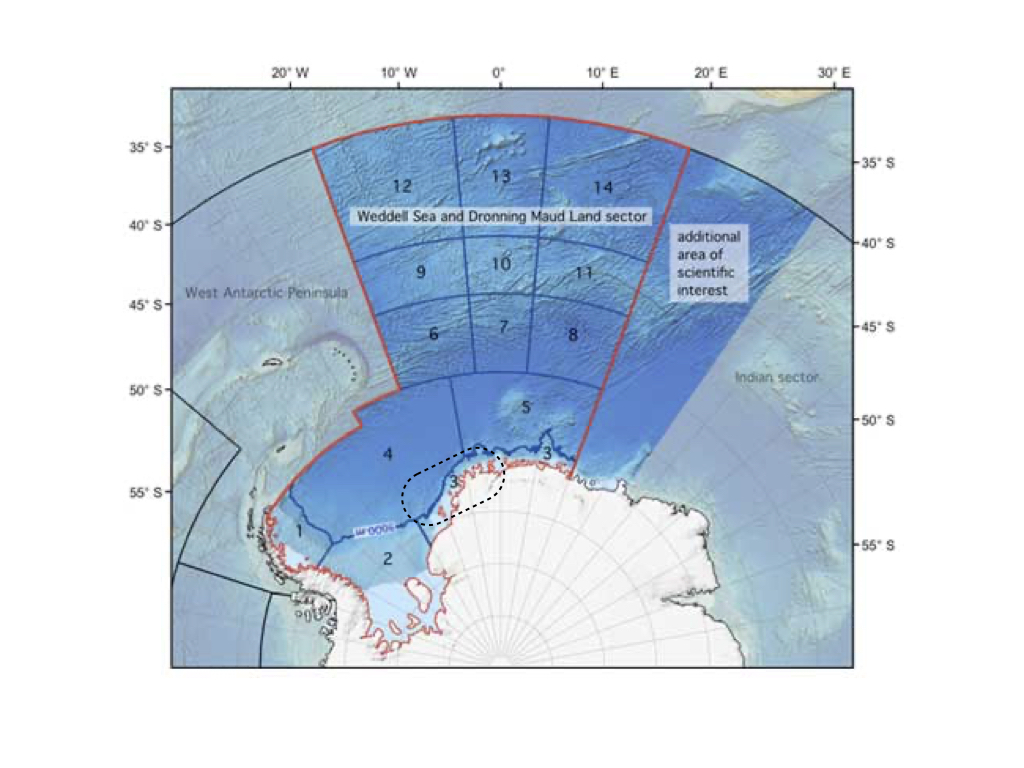
\includegraphics[width=12cm]{Fig.1_StudyMap} \caption{Map of the Weddell Sea and Dronning Maud Land sector highlighting the high Antarctic shelf as a dashed-line contour. Modified from www.soos.aq.}\label{fig:unnamed-chunk-1}
\end{figure}

\clearpage

\begin{figure}
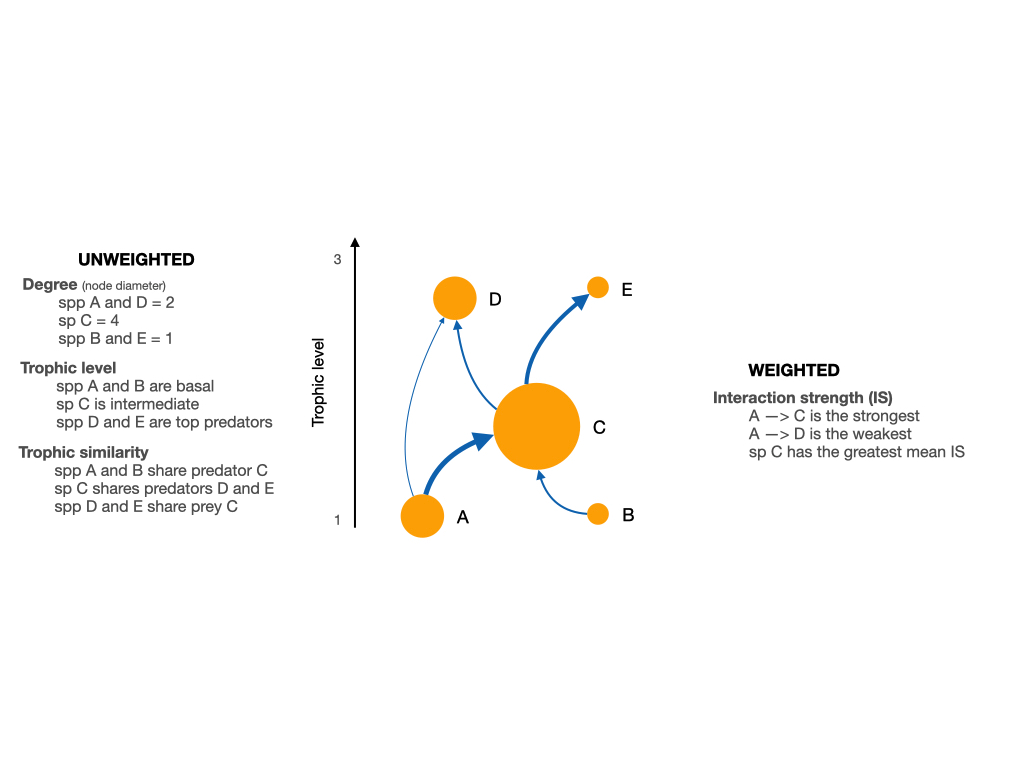
\includegraphics[width=12cm]{Fig.2_ToyFoodWeb} \caption{Scheme of a network showing the weighted and unweighted properties we used to characterize the species of the Weddell Sea food web.}\label{fig:unnamed-chunk-2}
\end{figure}

\clearpage

\begin{figure}
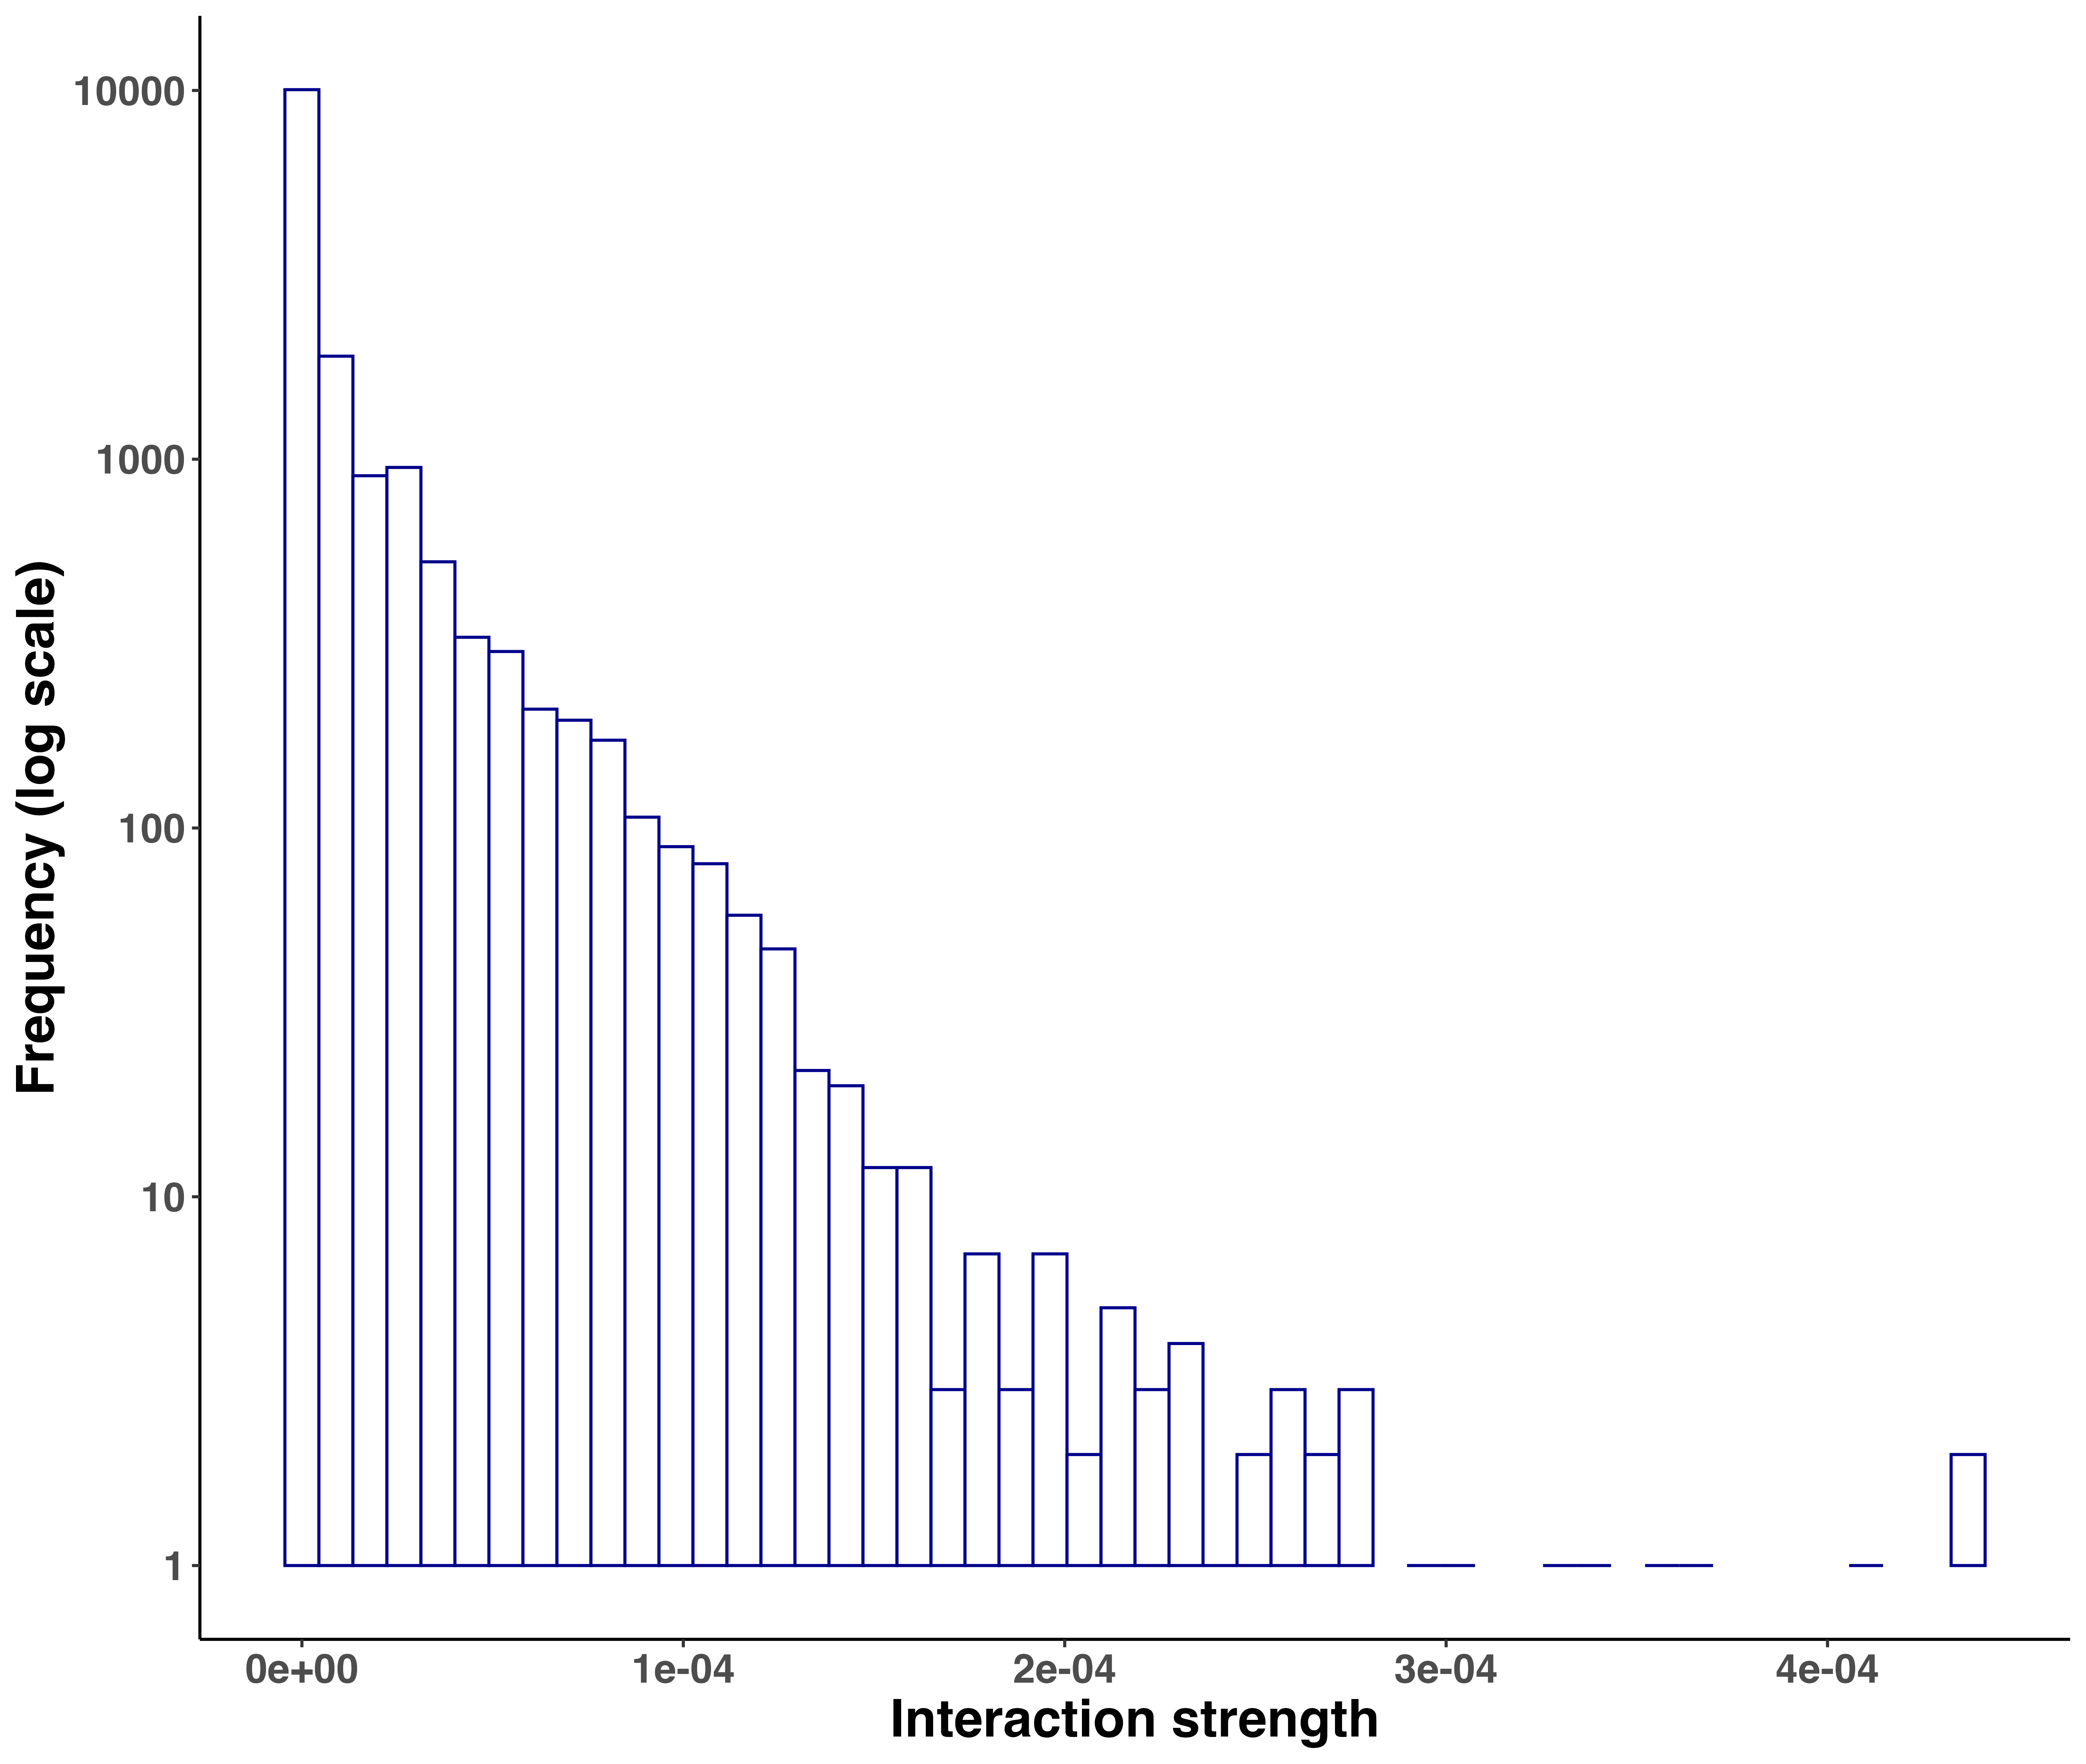
\includegraphics[width=12cm]{Fig3_IntDist} \caption{Frequency distribution of interaction strengths for the Weddell Sea food web (n = 490).}\label{fig:unnamed-chunk-3}
\end{figure}

\clearpage

\begin{figure}
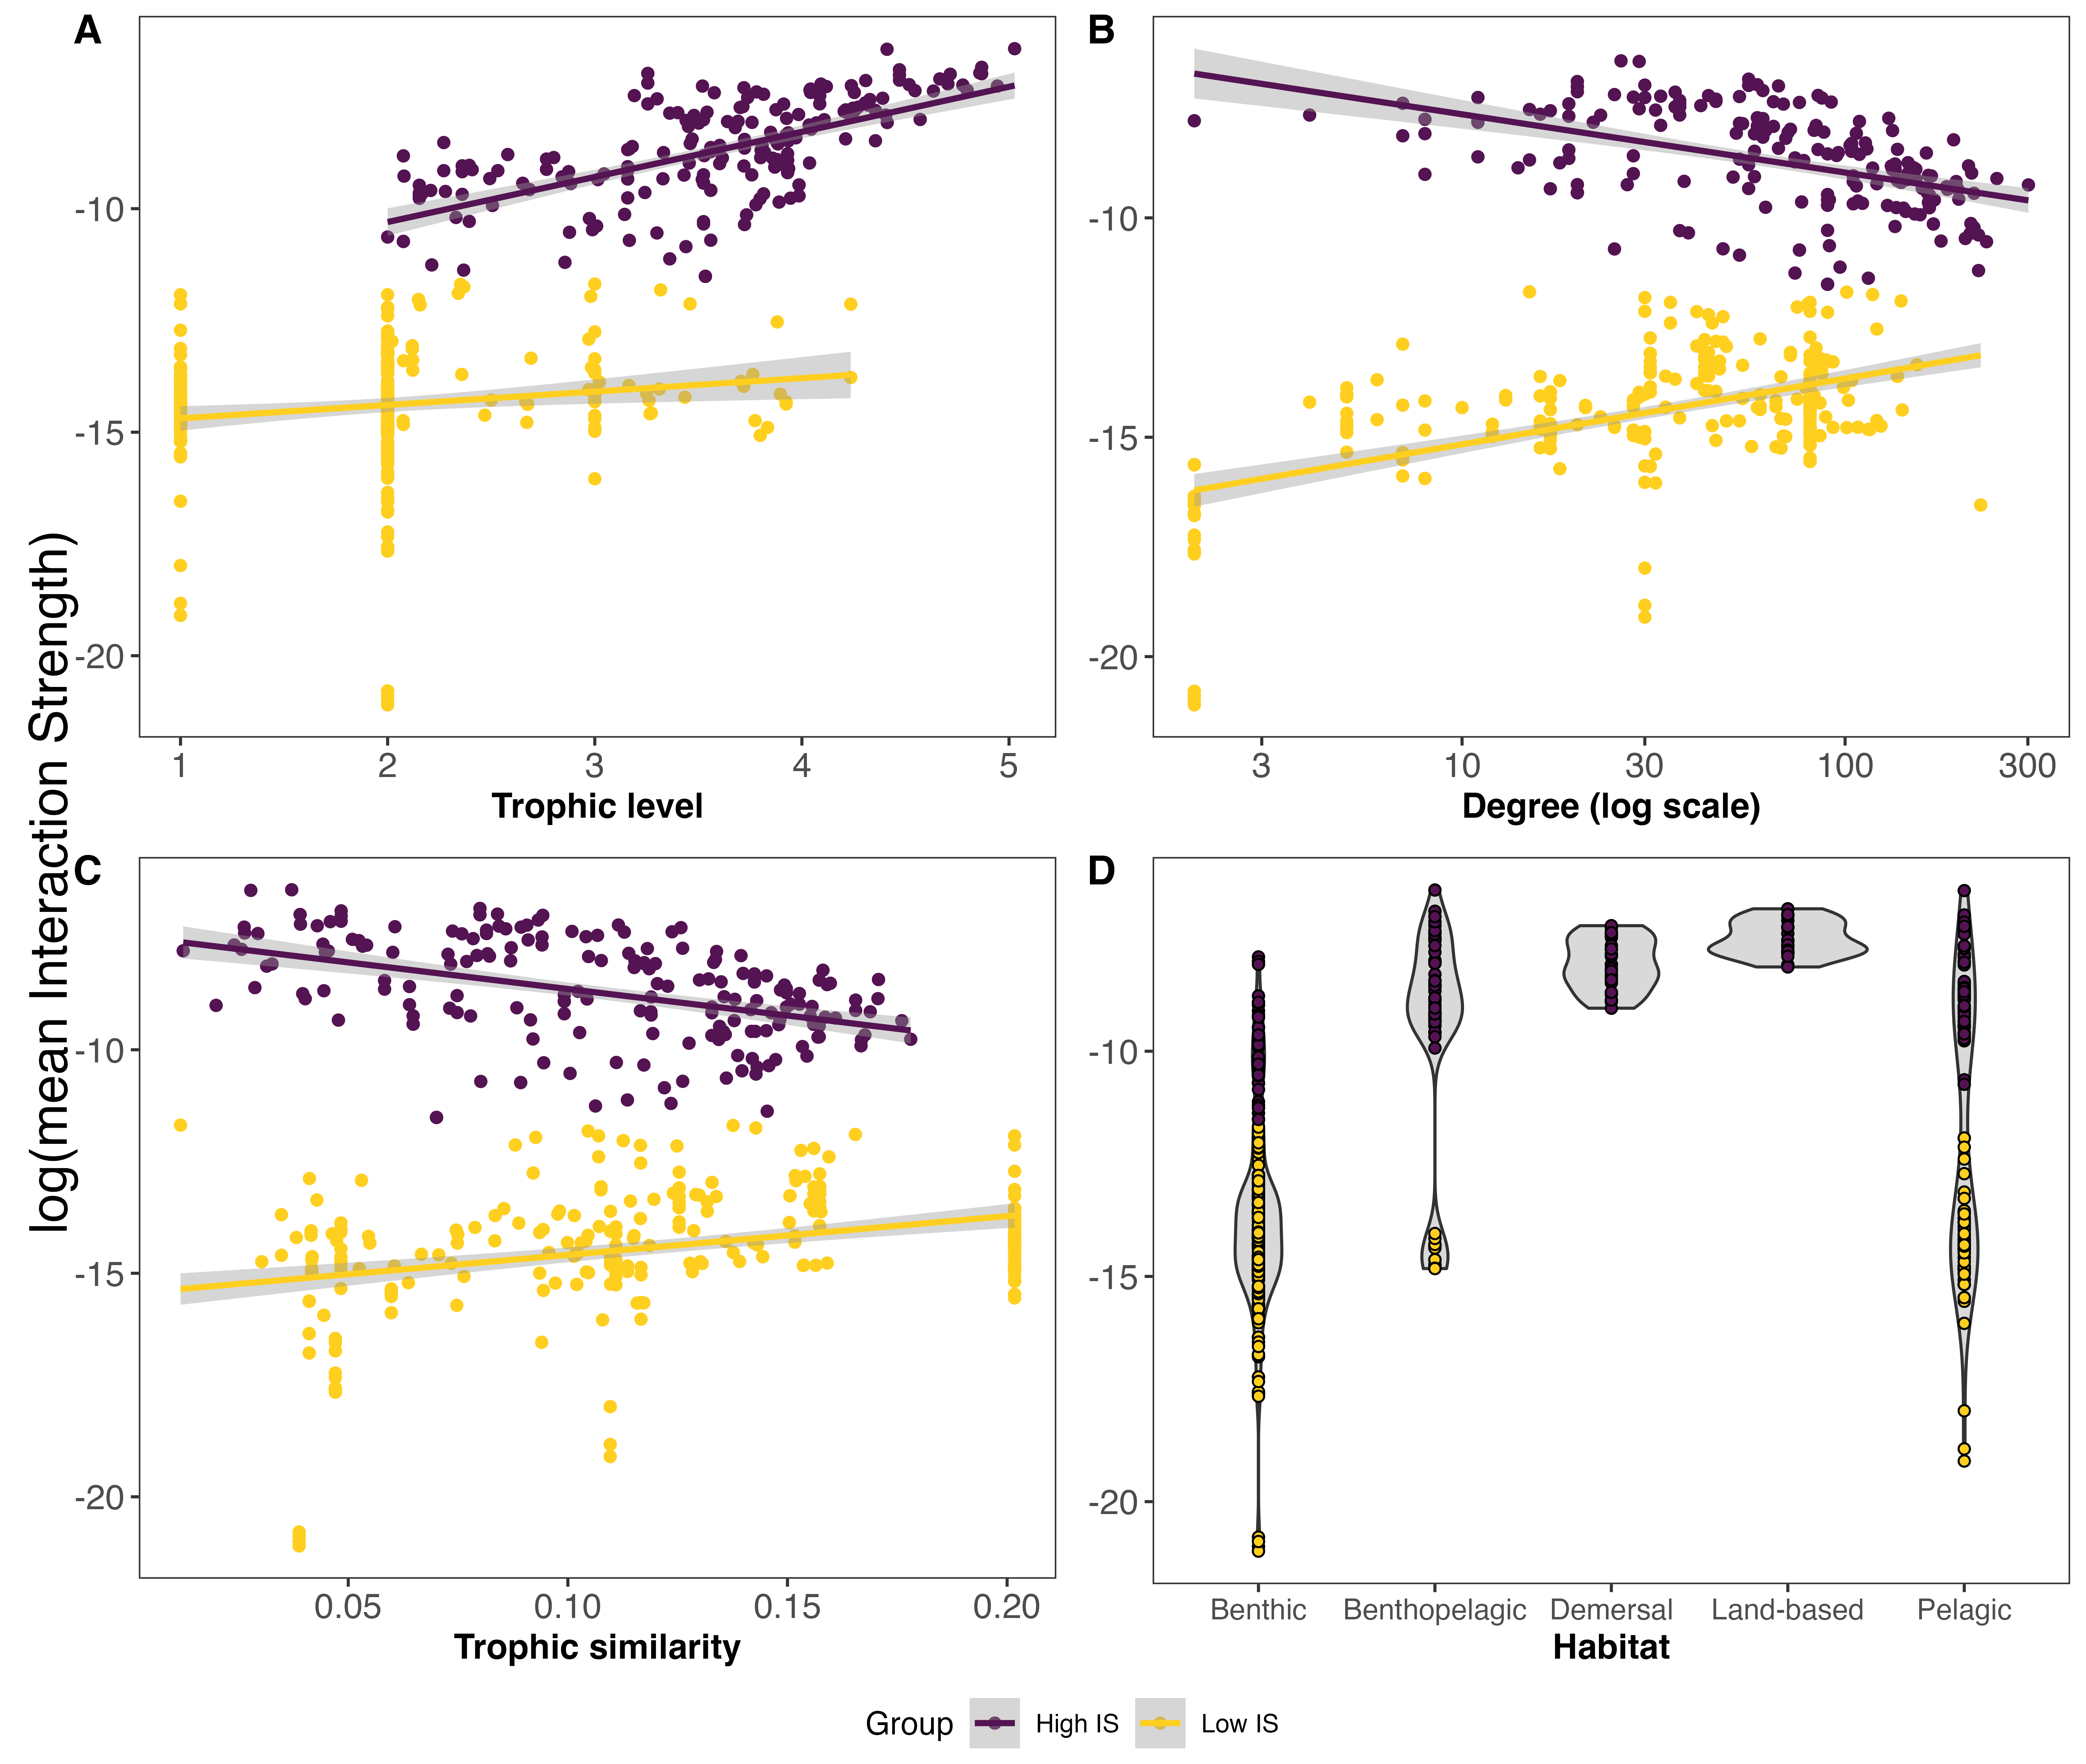
\includegraphics[width=12cm]{Fig4_LinReg} \caption{Relationships between weighted (mean Interaction Strength) and unweighted properties including habitat. Linear regressions are shown between log(mean interaction strength) and trophic level (A), degree (B) and trophic similarity (C). Equations for trophic level ($y = 1.12x - 15.29, R^2 = 0.43, p-value < 2e-16$), degree ($y = 0.006x - 12.77, R^2 = 0.03, p-value = 4.06e-5$) and trophic similarity ($y = -1.46x - 12.18, R^2 = -0.0004, p-value = 0.36$).}\label{fig:unnamed-chunk-4}
\end{figure}

\clearpage

\begin{figure}
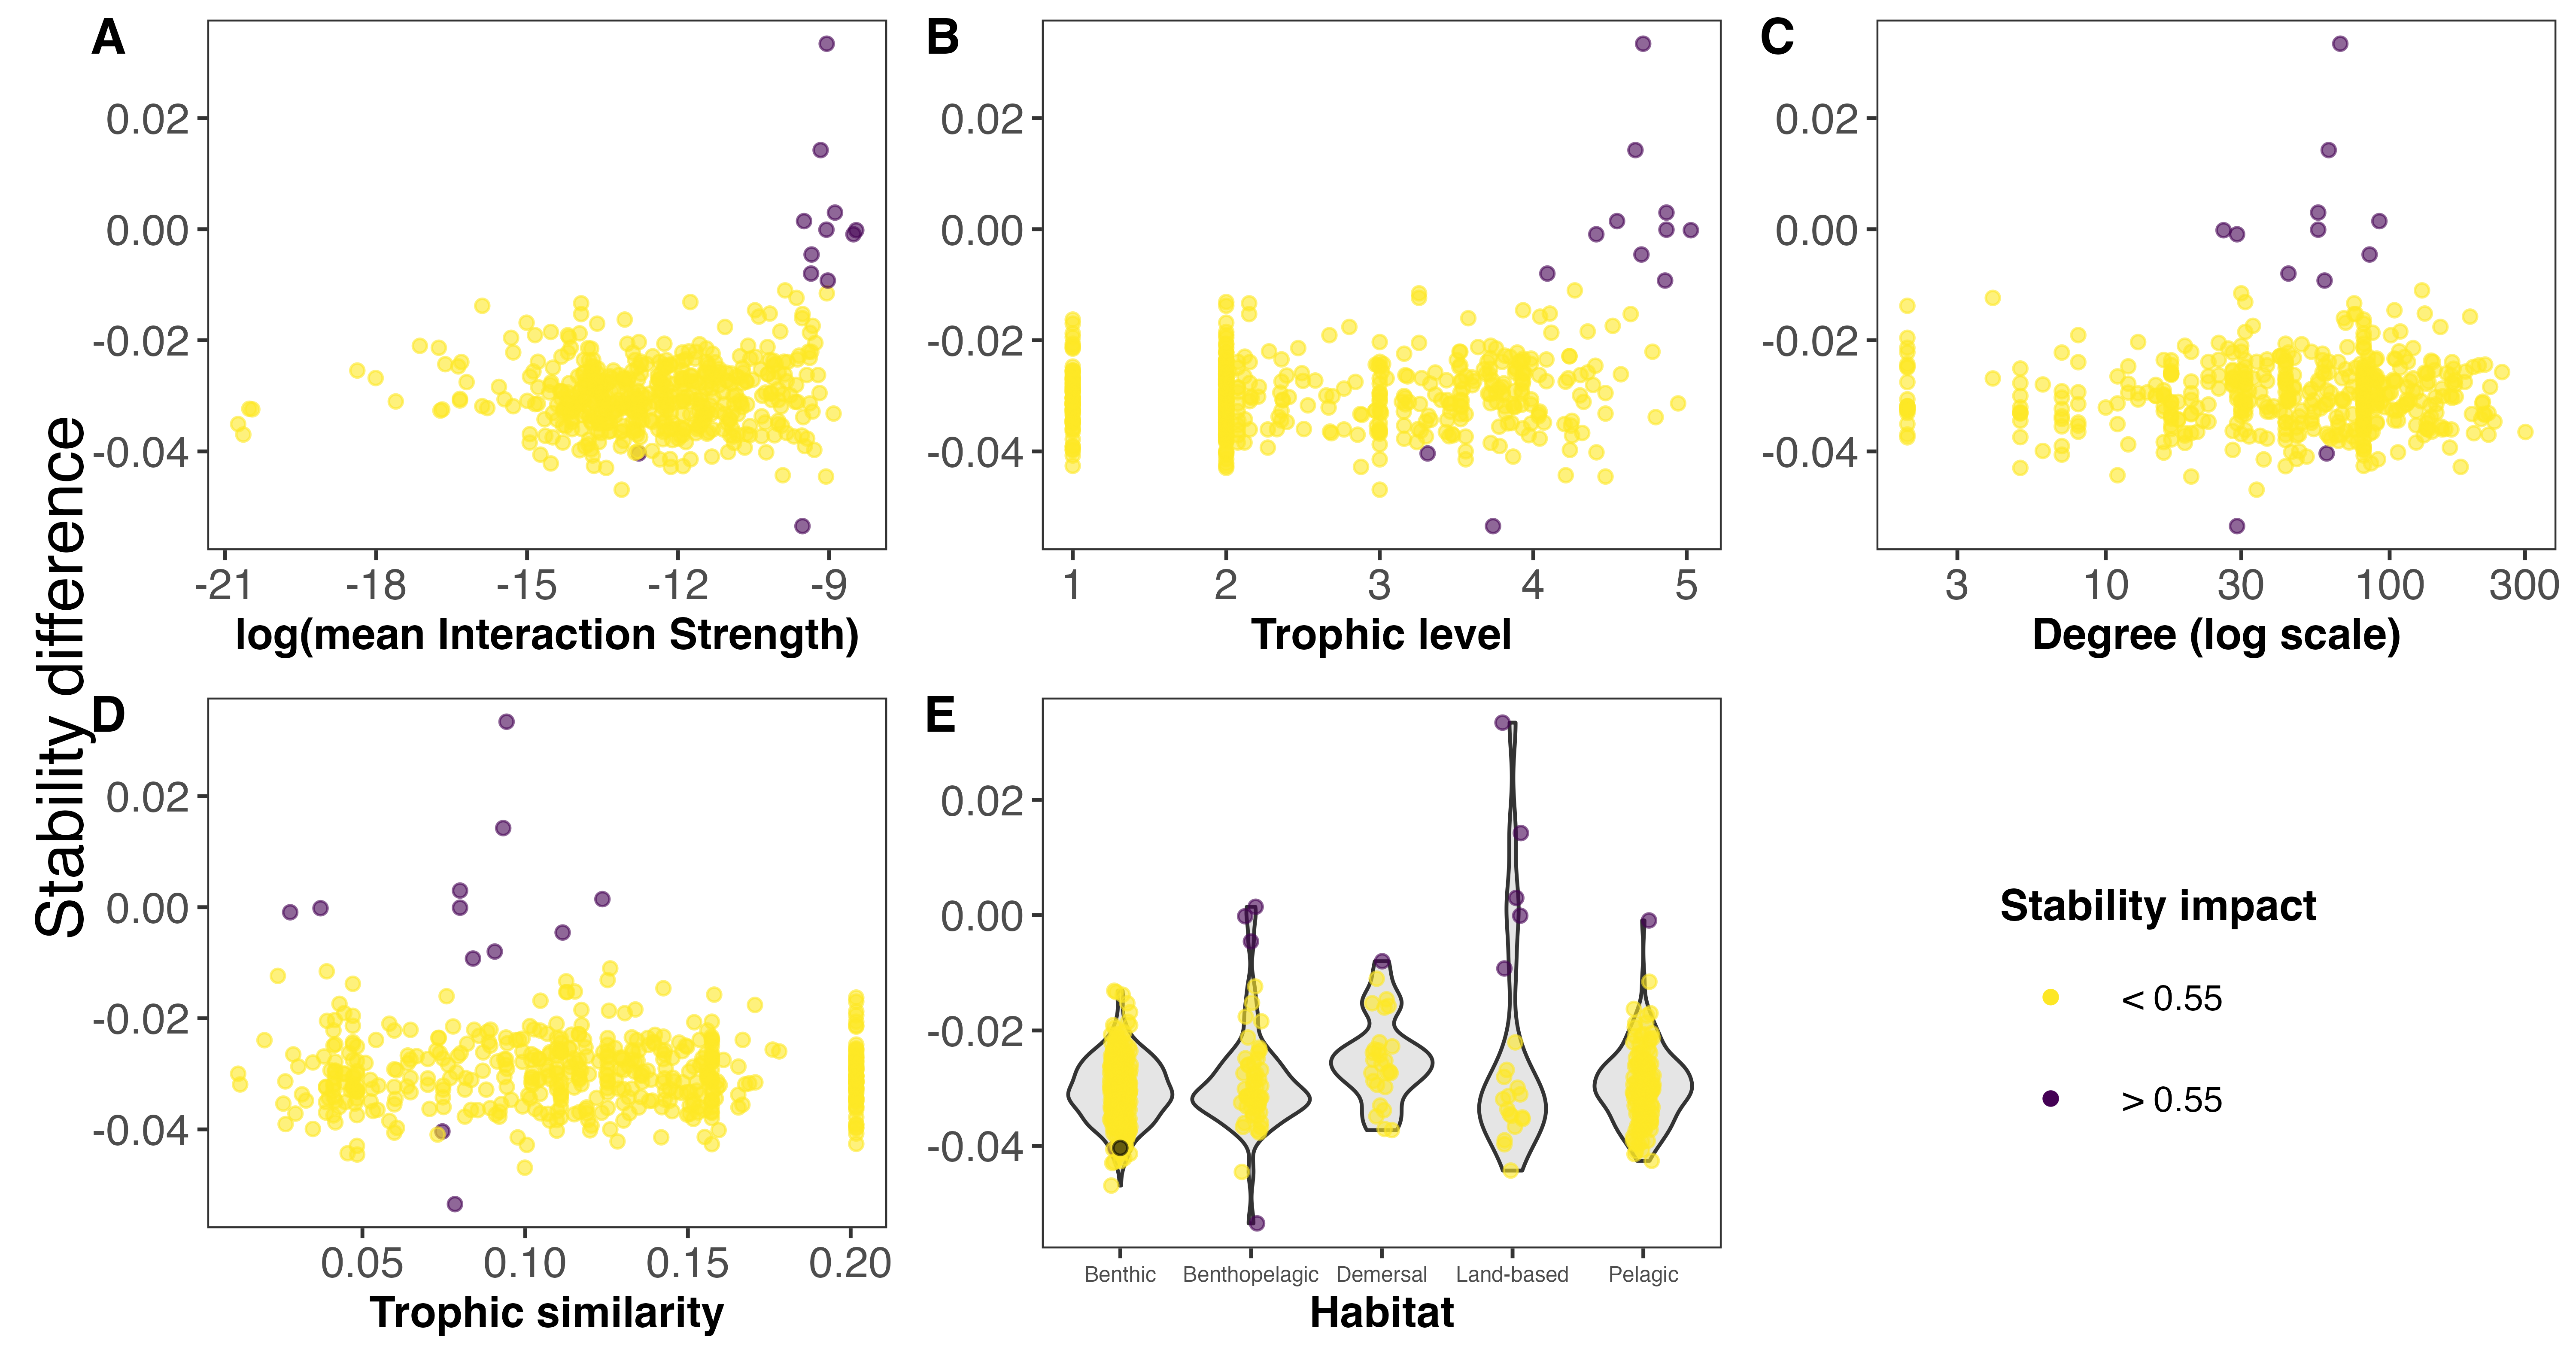
\includegraphics[width=12cm]{Fig.5_QSSDif} \caption{Quasi-Sign Stability (QSS) difference between the whole Weddell Sea food web (n = 490) and the food web without one species (n = 489) for weighted (interaction strength) and unweighted species properties, and habitat. Point color indicates the impact on the QSS; if significant the extinction of that species altered the stability of the food web.}\label{fig:unnamed-chunk-5}
\end{figure}

\clearpage

\begin{table}[t]
\caption{Model comparison for the distribution of interaction strengths of the Weddell Sea food web. Order by best fit. References: df = degrees of freedom, AIC = Akaike Information Criterion, deltaAIC = difference with best fit. Log-Normal is the best model.}
\begin{tabular}{l c c c}
\tophline

\textbf{Model} & \textbf{df} & \textbf{AIC} & \textbf{deltaAIC} \\
\middlehline
log-Normal & 2 & -359738 & 0 \\
\middlehline
Gamma & 2 & -359714.1 & 23.89 \\
\middlehline
Power-law & 2 & -350667 & 9070.97 \\
\middlehline
Exponential & 1 & -327606.5 & 32131.54 \\
\middlehline
Normal & 2 & -291407.8 & 68330.21 \\
\middlehline
Uniform & 2 & -248179 & 111559.02 \\

\bottomhline
\end{tabular}
\end{table}

\clearpage

\begin{table}[t]
\caption{Properties of the species that when become extinct generated a significant impact on the stability of the Weddell Sea food web, ordered by significance (Anderson-Darling p value). All species belong to the 'High IS' group.  References: meanIS = mean interaction strength, TL = trophic level, Deg = degree, TS = trophic similarity, StabDif = stability difference, ADvalue = Anderson-Darling p value.}
\begin{tabular}{l c c c c c c c}
\tophline

\textbf{Species} & \textbf{meanIS} & \textbf{TL} & \textbf{Deg} & \textbf{TS} & \textbf{Habitat} & \textbf{StabDif} & \textbf{ADvalue}\\
\middlehline
Orcinus orca & 1.83e-4 & 5.03 & 26 & 0.037 & Benthopelagic & 4.67e-5 & 2.28e-41 \\
\middlehline
Macrourus holotrachys & 8.30e-5 & 4.70 & 85 & 0.112 & Benthopelagic & 3.55e-5 & 2.73e-23 \\
\middlehline
Pagetopsis macropterus & 7.08e-5 & 4.64 & 76 & 0.113 & Demersal & -1.80e-5 & 2.38e-12 \\
\middlehline
Abyssorchomene nodimanus & 2.56e-5 & 4.21 & 137 & 0.130 & Benthopelagic & 2.30e-5 & 8.52e-10 \\
\middlehline
Dissostichus mawsoni & 7.82e-5 & 4.12 & 87 & 0.126 & Pelagic & 2.17e-5 & 1.57e-9 \\
\middlehline
Macrourus whitsoni & 7.14e-5 & 4.55 & 92 & 0.124 & Benthopelagic & 2.12e-5 & 3.30e-8 \\
\middlehline
Hydrurga leptonyx & 1.03e-4 & 4.72 & 67 & 0.094 & Land-based & 2.04e-5 & 9.66e-6 \\
\middlehline
Mesonychoteuthis hamiltoni & 1.80e-4 & 4.41 & 29 & 0.028 & Pelagic & 1.82e-5 & 4.59e-5 \\
\middlehline
Champsocephalus gunnari & 7.62e-5 & 3.72 & 46 & 0.086 & Pelagic & 1.83e-5 & 6.79e-5 \\
\middlehline
Notothenia marmorata & 8.27e-5 & 4.09 & 44 & 0.091 & Demersal & 1.60e-5 & 1.23e-4 \\
\middlehline
Arctocephalus gazella & 9.28e-5 & 4.67 & 61 & 0.093 & Land-based & 1.17e-5 & 2.09e-4 \\
\middlehline
Trematomus pennellii & 3.04e-5 & 4.04 & 192 & 0.158 & Demersal & 1.44e-5 & 1.00e-3 \\
\middlehline
Mirounga leonina & 1.20e-4 & 4.87 & 56 & 0.080 & Land-based & 1.41e-5 & 1.28e-3 \\
\middlehline
Notothenia coriiceps & 4.94e-5 & 4.27 & 130 & 0.126 & Demersal & 1.44e-5 & 1.66e-3 \\
\middlehline
Maxilliphimedia longipes & 2.21e-6 & 3.26 & 60 & 0.136 & Benthopelagic & -4.46e-6 & 9.74e-3 \\

\bottomhline
\end{tabular}
\end{table}

\appendixfigures
\clearpage

\begin{figure}
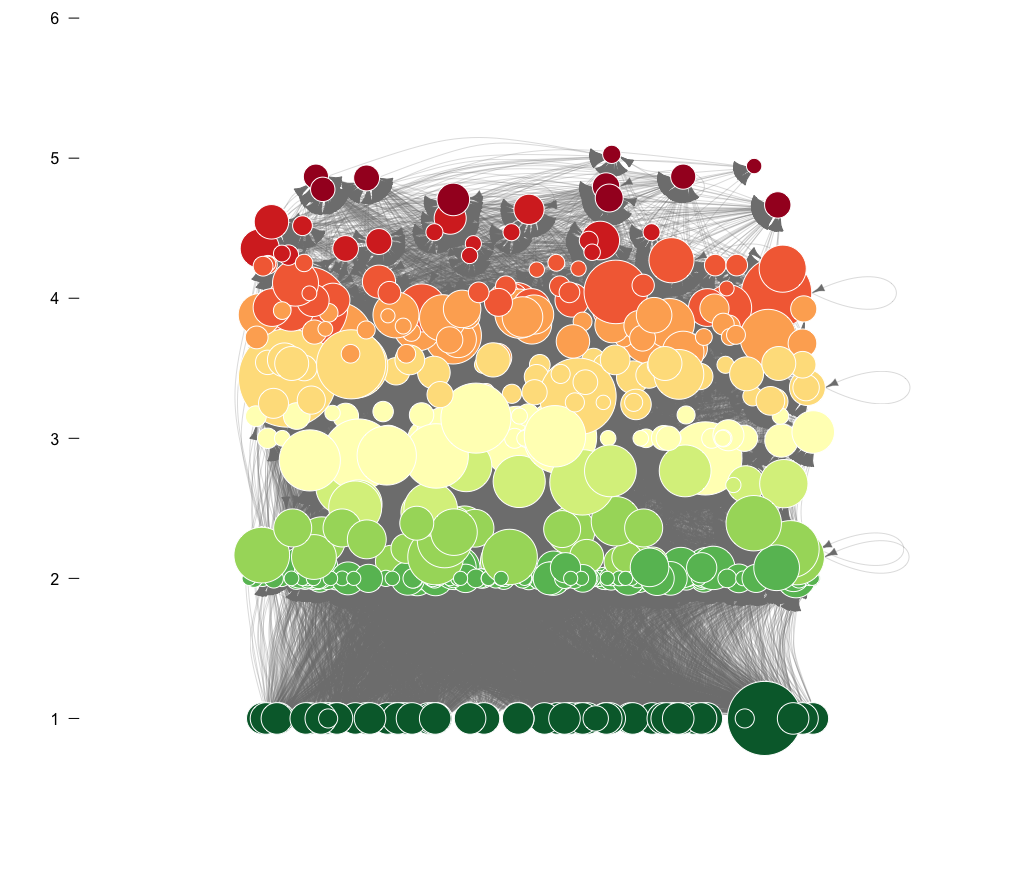
\includegraphics[width=12cm]{App1_FWplot} \caption{Graphic representation of the Weddell Sea food web. Species (nodes) are arranged vertically and colored by trophic level. The diameter of the node indicates the total number of interactions. Predator-prey interactions are represented by the arrows, from prey to predator.}\label{fig:unnamed-chunk-6}
\end{figure}






%%%%%%%%%%%%%%%%%%%%%%%%%%%%%%%%%%%%%%%%%%
%% optional

%%%%%%%%%%%%%%%%%%%%%%%%%%%%%%%%%%%%%%%%%%

%%%%%%%%%%%%%%%%%%%%%%%%%%%%%%%%%%%%%%%%%%
\authorcontribution{TIM and LAS: Conceptualization (lead); Data curation
(lead); Formal analysis (lead); Methodology (lead); Coding (lead);
Writing -- original draft (lead); Writing -- review and editing (lead).
SK: Conceptualization (lead); Formal analysis (supporting); Methodology
(supporting); Coding (supporting); Writing -- original draft
(supporting); Writing -- review and editing
(supporting).} %% optional section

%%%%%%%%%%%%%%%%%%%%%%%%%%%%%%%%%%%%%%%%%%
\competinginterests{The authors declare no competing
interests.} %% this section is mandatory even if you declare that no competing interests are present

%%%%%%%%%%%%%%%%%%%%%%%%%%%%%%%%%%%%%%%%%%

%%%%%%%%%%%%%%%%%%%%%%%%%%%%%%%%%%%%%%%%%%
\begin{acknowledgements}
Thanks to the rticles contributors!
\end{acknowledgements}

%% REFERENCES
%% DN: pre-configured to BibTeX for rticles

%% The reference list is compiled as follows:
%%
%% \begin{thebibliography}{}
%%
%% \bibitem[AUTHOR(YEAR)]{LABEL1}
%% REFERENCE 1
%%
%% \bibitem[AUTHOR(YEAR)]{LABEL2}
%% REFERENCE 2
%%
%% \end{thebibliography}

%% Since the Copernicus LaTeX package includes the BibTeX style file copernicus.bst,
%% authors experienced with BibTeX only have to include the following two lines:
%%
\bibliographystyle{copernicus}
\bibliography{../WeddellSea.bib}
%%
%% URLs and DOIs can be entered in your BibTeX file as:
%%
%% URL = {http://www.xyz.org/~jones/idx_g.htm}
%% DOI = {10.5194/xyz}


%% LITERATURE CITATIONS
%%
%% command                        & example result
%% \citet{jones90}|               & Jones et al. (1990)
%% \citep{jones90}|               & (Jones et al., 1990)
%% \citep{jones90,jones93}|       & (Jones et al., 1990, 1993)
%% \citep[p.~32]{jones90}|        & (Jones et al., 1990, p.~32)
%% \citep[e.g.,][]{jones90}|      & (e.g., Jones et al., 1990)
%% \citep[e.g.,][p.~32]{jones90}| & (e.g., Jones et al., 1990, p.~32)
%% \citeauthor{jones90}|          & Jones et al.
%% \citeyear{jones90}|            & 1990


\end{document}
